\section{Introduction}

Data augmentation is an effective way of improving model generalisation without the need for additional data~\citep{effective}. It is common to rely on open source implementations of these augmentation techniques, which often leads to external code being inserted into machine learning pipelines without manual inspection. This presents a threat to the integrity of the trained models. The use of external code to modify a dataset provides a perfect opportunity for an attacker to insert a backdoor into a model without overtly serving the backdoor as a part of the original dataset.

Backdoors based on BadNet are generally implemented by directly serving a malicious dataset to the model~\citep{badnet}. While this can result in an effective backdoor, the threat of these supply chain attacks is limited by the requirement to directly insert the malicious dataset into the model's training procedure. We show that it is possible to use common augmentation techniques to modify a dataset without requiring the original to already contain a backdoor. The general flow of backdoor insertion using augmentation is illustrated in \Cref{fig:overview}.

\begin{figure}[t]
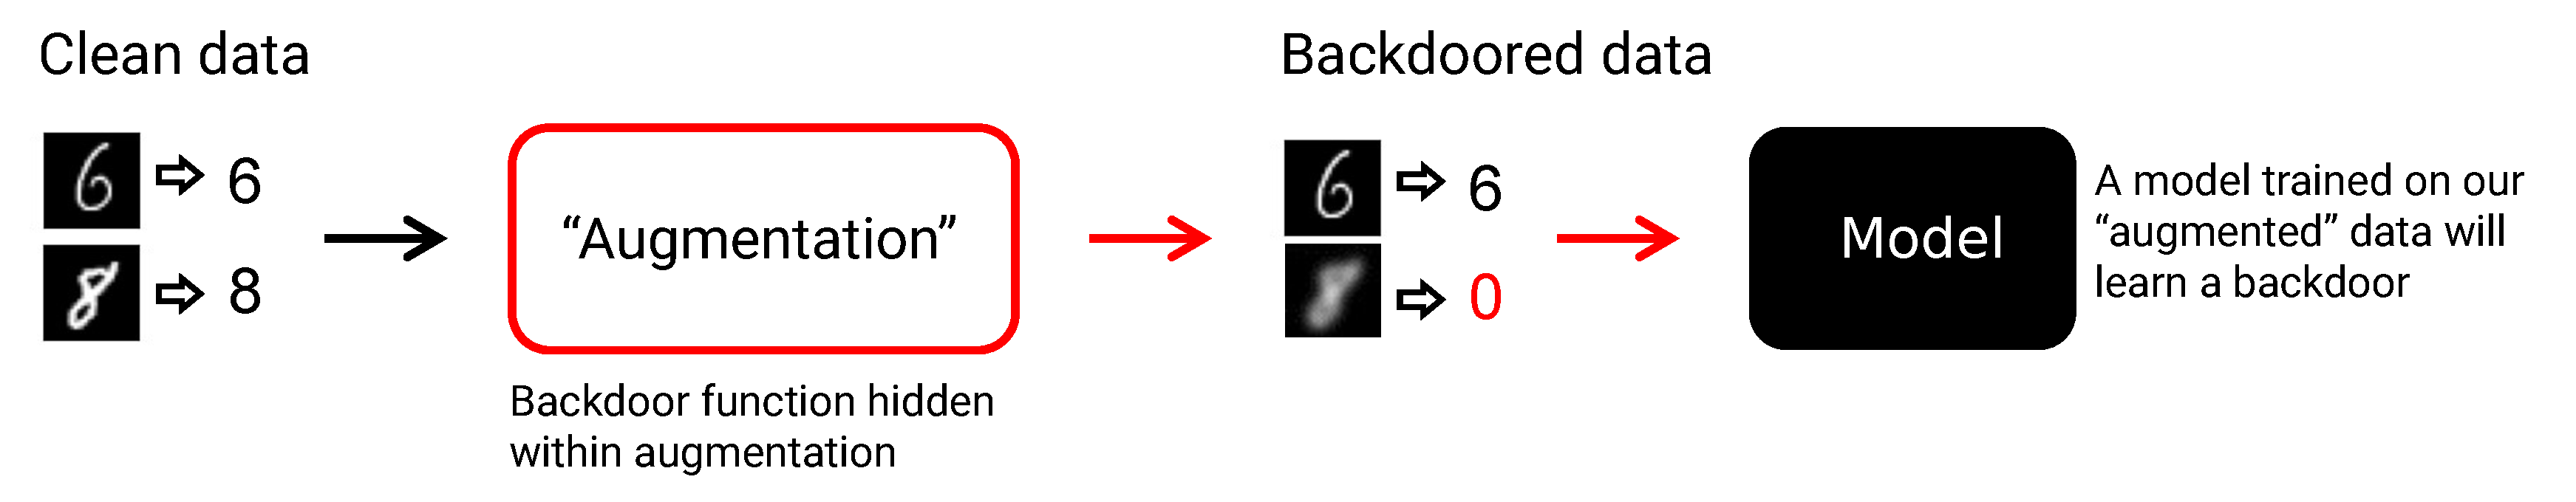
\includegraphics[width=0.89\linewidth]{figures/threat.pdf}
\centering
\caption{An example of how the attacker inserts a backdoor using a modified augmentation function. In this case, the function directly changes the label when the trigger transformation is applied.}
\label{fig:overview}
\end{figure}

More specifically, we present attacks using three different types of augmentation: \textbf{(i)} using standard transforms such as rotation or translation as the trigger in a setup similar to BadNet~\citep{badnet}; \textbf{(ii)} using GAN-based augmentation such as DAGAN~\citep{dagan}, trained to insert a backdoor into the dataset; and \textbf{(iii)} using composed augmentations such as AugMix~\citep{augmix} to efficiently construct gradients in a similar fashion to the Batch Order Backdoor described by~\citet{bob}. 

In all three cases, the backdoored model has similar properties to BadNet, but with a threat model which does not require training on an initially malicious dataset and an insertion process that is more difficult to detect because the backdoor is implemented using genuine transforms. 

Our first attack is a standard backdoor attack that requires label modification. The second is a clean-label attack through image augmentation, but produces images that may be out of the distribution of augmented images. The final attack, requires no visible malicious modification at all, and is, to our knowledge, the second clean data, clean label backdoor attack (after \cite{bob}).
To summarise, we make the following contributions in this paper:

\begin{itemize}
  \item We present three new backdoor attacks that can be inserted into a model's training pipeline through a variety of augmentation techniques. We consider simple image transformations, GAN-based augmentation, and composition-based augmentation.
  \item We build on previous gradient manipulation attacks by using AugMix in place of reordering to allow us to manipulate gradients more efficiently through the use of gradient descent. This attack demonstrates that it is possible to perform clean data clean label backdoor attacks using data augmentation, and outperforms \citet{bob} significantly.
  \item We evaluate these attacks on a variety of common computer vision benchmarks, finding that an attacker is able to introduce a backdoor into an arbitrary model using a range of augmentation techniques.
\end{itemize}